% siminos/spatiotemp/chapter/action.tex
% $Author: predrag $ $Date: 2021-12-24 01:25:20 -0500 (Fri, 24 Dec 2021) $

% \ifblog  Predrag 2021-06-12 gave up on this,
%          do not remember who calls it other than blogCats.tex
    \chapter{Hill's formula}
    \label{c-Hill}  % temporary, while being edited in spatiotemp/
%\renewcommand{\cl}[1]{{\ensuremath{n_{#1}}}}   % discrete length of a cycle, Predrag
\renewcommand{\shift}{\ensuremath{\ell}}

\section{An overview over ``Hill's formulas''}
\label{sect:Hill}
%\renewcommand{\cl}[1]{{\ensuremath{|#1|}}}  % the length of a periodic orbit, Ronnie
\renewcommand{\shift}{\ensuremath{d}}

\begin{quote}
A succinct  explanation of the Hill's formula:\\
If you evaluate stability of the 3-term recurrence \refeq{JiKoKr20(2)} on
a periodic lattice you get the {\jacobianOrb} $\jMorb$;
if you evaluate it by multiplying the `two-configuration representation'
matrix $\jMps$, you get the `time evolution' side of the Hill's formula.
\end{quote}

We should emphasize that, while discovered first in Lagrangian setting,
Hill's formulas are much more general, they
apply also to dissipative dynamical systems as well, see

CL18 \HREF{http://chaosbook.org/~predrag/papers/CL18.pdf\#subsection.1.5}
{sect.~1.5} {\em  Stability of an orbit vs.  its time-evolution stability}

CL18 \HREF{http://chaosbook.org/~predrag/papers/CL18.pdf\#appendix.C}
{appendix~C} {\em Spatiotemporal stability}


\refsect{LiTom17b:GenFctn} {\em Generating functions; action}
%\else  Predrag 2021-06-12 gave up on this,
%          do not remember who calls it other than blogCats.tex
%\subsection{Generating functions; action}
%\fi


\refsect{sect:HillLagr} {\em Hill's formula, Lagrangian setting}


\refsect{sect:catlattHill} {\em \catLatt\ Hill's formula}


\refsect{sect:catlattHillrel} {\em Hill's formula for \rpo s}


\refsect{sect:templattHillHan} {\em Han's \templatt\ Hill's formula}


\refsect{sect:catlattHillHan} {\em Han's  \catlatt\ Hill's formula}


\refsect{sect:catlattHillRelativeHan} {\em Han's relative-periodic Hill's formula}


\refsect{sect:HenonHillHan} {\em Han's  \HenonMap\ Hill's formula}











\section{Generating functions; action}
%\else  Predrag 2021-06-12 gave up on this,
%          do not remember who calls it other than blogCats.tex
%\subsection{Generating functions; action}
%\fi
\label{LiTom17b:GenFctn}

    \PC{2016-11-11, 2018-09-26}{
What follows is (initially)
copied from Li and Tomsovic\rf{LiTom17b}, \emph{Exact relations between
homoclinic and \po\ actions in chaotic systems} arXiv source
file, then merged with the MacKay-Meiss-Percival action
principle \refrefs{MKMP84,meiss92}.
    }
For discrete-time one-degree-of-freedom Lagrangian systems satisfying a
periodicity condition (\ie, cat map):
\beq
\genF(\coord+1, \coord'+1)=\genF(\coord, \coord')+C
\,,
\ee{MacMei83-2}
one can consider relative periodic paths (or pre-periodic paths, also called
periodic paths of type $(\shift,\cl{})$ by Mackay and Meiss\rf{MacMei83}), with
    \PC{2018-09-29} {presumably they are \rpo s, or pre-\po s, with a rational
    winding number $p/\coord$.}
\beq
\coord_{i+\cl{}}=\coord_{i}+\shift
\,.
\ee{MacMei83-3}
Every $\coord_{i}$ returns to its value after time period $\cl{}$, but shifted by
$\shift$.
Orbits satisfying \refeq{MacMei83-3} are given by stationary points of the action
\beq
\action = \sum_{i=0}^{q-1} \genF(\coord_i, \coord_{i+1})
\ee{MacMei83-4}
in the space of periodic paths of type $(\shift,\cl{})$.
For periodic paths, it suffices to consider one period, because an orbit is periodic if
and only if it is a stationary point of the action of one period in the space
of periodic paths.

If the constant $C$ (the
\HREF{https://floerhomology.wordpress.com/2015/09/14/mean-action-and-the-calabi-invariant/}
{Calabi invariant}\rf{Calabi70}) in the periodicity condition
\refeq{MacMei83-2} is zero, and the Lagrangian satisfies a convexity
condition
\beq
\genF_{12}(\coord, \coord') < 0
\,,
\ee{MacMei83-5}
where subscript $k$ refers to the derivative with respect to the $k$th
argument, then the action of periodic paths of type  $(\shift,\cl{})$ is bounded below,
so there is a minimising path. Since its action is stationary, it gives a \po\
of type  $(\shift,\cl{})$.

    \PC{2018-01-21}{Is this true?
To go from the Hamiltonian $(\ssp_{\zeit},p_{\zeit})$ phase space formulation to the
Newtonian (or Lagrangian) $(\ssp_{\zeit-1},\ssp_{\zeit})$ {\em state space}
formulation, replace $p_\zeit$  by
\(
p_\zeit = (\ssp_{\zeit} - \ssp_{\zeit-1})/\Delta\zeit \,,
\)
where $\Delta\zeit =1$.
    }
    %
For {\orbit} ${p}$  of period $\cl{p}$, the {action} of the \orbit\ is:
\beq
\label{eq:DefGenFprimePOs}
\action_{p}  \equiv \sum_{n=0}^{\cl{p}-1}\genF(\coord_{n},\coord_{n+1})\ .
\eeq
$\action_{p}$ is the generating function that maps a point along the orbit for one
(prime) period.  For the case of a fixed point $p$ of period $\cl{p}=1$,
the action is
\beq\label{eq:Definition generating function fixed points}
\action_{p}  = \genF(\coord_p,\coord_p)
\,,
\eeq
where the generating function $\genF(\coord_p,\coord_p)$ maps $\ssp_p$ into itself in one
iteration.

\section{Homoclinic and \po\ actions in chaotic systems}

    \PC{2018-09-29}{
What follows is copied from Li and Tomsovic\rf{LiTom17b}.
    }
For an aperiodic orbit $\lbrace\ssp_0\rbrace$ going through the point $\ssp_0$,
the action, evaluated as the sum over an infinity of successive mappings,
\begin{equation}
\label{eq:full orbit action in general}
\action_{\lbrace \ssp_0 \rbrace}
\equiv \lim_{N \to \infty}
\sum_{n=-N}^{N-1} \genF(\coord_{n},\coord_{n+1})
=\lim_{N \to \infty} \action_{-N,N}
\,,
\end{equation}
is not necessarily convergent. However, the MacKay-Meiss-Percival action
principle\rf{MKMP84,meiss92} can be applied to obtain well defined
action differences between pairs of orbits.  For example,
the {\em relative} {\em action}
$\Delta \action_{\lbrace h_0 \rbrace  \lbrace x \rbrace}$ between a fixed point $\ssp_p$
and its homoclinic orbit $\lbrace h_{0} \rbrace$, where $h_{\pm
\infty}\to \ssp_p$:
\begin{eqnarray}
\label{eq:relative action homoclinic}
\Delta \action_{\lbrace h_0 \rbrace  \lbrace \ssp_p \rbrace}
 &\equiv & \lim_{N \to \infty} \sum_{i=-N}^{N-1}\left[\genF(h_i,h_{i+1})-\genF(\ssp_p,\ssp_p)\right]
\nonumber \\
&=& \int\limits_{U[\ssp_p,h_{0}]}p\mathrm{d}\coord+\int\limits_{S[h_{0},\ssp_p]}p\mathrm{d}\coord
= \oint_{US[\ssp_p,h_{0}]} p\mathrm{d}\coord \nonumber \\
&=& {\cal A}^\circ_{US[\ssp_p,h_{0}]}
\end{eqnarray}
where $U[\ssp_p,h_{0}]$ is the segment of the unstable manifold from $\ssp_p$ to
$h_{0}$, and $S[h_{0},\ssp_p]$ the segment of the stable manifold from $h_0$
to $\ssp_p$.  The $\circ$ superscript on the last line indicates that the area
is interior to a path that forms a closed loop, and the subscript
indicates the path: $US[\ssp_p,h_{0}]=U[\ssp_p,h_{0}]+S[h_{0},\ssp_p]$.  The
clockwise enclosure of an area is positive, counterclockwise negative.
$\Delta \action_{\lbrace h_0 \rbrace \lbrace \ssp_p \rbrace} $ gives the
action difference between the homoclinic orbit segment $[
h_{-N},\cdots,h_{N} ]$ and the length-$(2N+1)$ fixed point orbit segment
$[ \ssp_p, \cdots, \ssp_p ]$ in the limit $N \to \infty$. In later sections, upon
specifying the symbolic code of the homoclinic orbit $\lbrace h_0 \rbrace
\Rightarrow \overline{0} \gamma \overline{0}$, we also denote $\Delta
\action_{\lbrace h_0 \rbrace  \lbrace \ssp_p \rbrace}$ alternatively as
\begin{equation}\label{eq:relative action homoclinic symbolic notation}
\Delta \action_{\lbrace h_0 \rbrace  \lbrace \ssp_p \rbrace}
= \Delta \action_{\overline{0} \gamma \overline{0},  \overline{0}}
\end{equation}
by replacing the orbits in the subscript with their symbolic codes.

%%%%%%%%%%%%%%%%%%%%%%%%%%%%%%%%%%%%%%%%%%%%%%%%%%%%%%%%%%%%%%%%%%%%%
\begin{figure}
   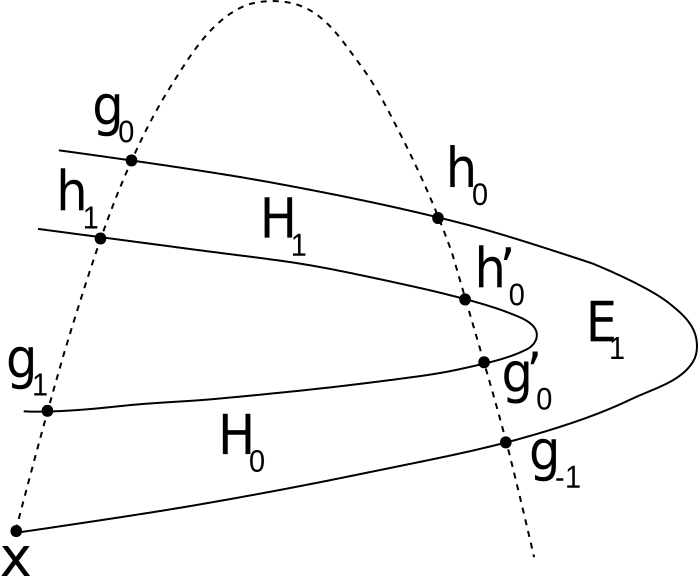
\includegraphics[width=0.5\textwidth]{LiTom17bHorseshoe2}
\caption{\label{fig:Horseshoe2}
A sketch of a partial homoclinic tangle
which forms a complete horseshoe structure. The unstable (stable)
manifold of $x$ is the solid (dashed) curve. There are two primary
homoclinic orbits $\lbrace h_0\rbrace$ and $\lbrace g_0\rbrace$.
$\cal{R}$ is the closed region bounded by loop
$\mathcal{L}_{USUS[x,g_{-1},h_0,g_0]}$.
~(From \refref{LiTom17b})
        }
\end{figure}
%%%%%%%%%%%%%%%%%%%%%%%%%%%%%%%%%%%%%%%%%%%%%%%%%%%%%%%%%%%%%%%%%%%%%

Likewise, a second important case is for the relative action between a
pair of homoclinic orbits $\lbrace h^{\prime}_0\rbrace \Rightarrow
\overline{0} \gamma^{\prime} \overline{0} $ and $\lbrace h_0\rbrace
\Rightarrow \overline{0} \gamma \overline{0}$, which results in
\begin{eqnarray}
\label{eq:homoclinic action difference}
\Delta \action_{{\lbrace h^{\prime}_0\rbrace}{\lbrace h_0\rbrace}} &\equiv & \lim_{N \to \infty} \sum_{i=-N}^{N-1}\left[ \genF(h^{\prime}_{i},h^{\prime}_{i+1}) - \genF(h_{i},h_{i+1})\right] \nonumber \\
& = & \lim_{N \to \infty} \left[ \genF(h^{\prime}_{-N},h^{\prime}_{N}) - \genF(h_{-N},h_{N}) \right] \nonumber \\
& = & \int\limits_{U[h_{0},h^\prime_{0}]}p\mathrm{d}\coord+\int\limits_{S[h^\prime_{0},h_{0}]}p\mathrm{d}\coord =  {\cal A}^\circ_{US[h_0,h^\prime_{0}]} \nonumber \\
& = & \Delta \action_{ \overline{0} \gamma^{\prime} \overline{0},  \overline{0} \gamma \overline{0} }
\end{eqnarray}
where $U[h_{0},h^\prime_{0}]$ is the segment of the unstable manifold
from $h_{0}$ to $h^\prime_{0}$, and $S[h^\prime_{0},h_{0}]$ the segment
of the stable manifold from $h^\prime_{0}$ to $h_{0}$.  Due to the fact
that the endpoints approach $\ssp_p$ forward and backward in time, one can
also write
\begin{eqnarray}
\label{eq:homoclinic action difference2}
\Delta \action_{{\lbrace h^{\prime}_0\rbrace}{\lbrace h_0\rbrace}}
& = & \lim_{N \to \infty}
\left[ \genF(h^{\prime}_{-(N+n)},h^{\prime}_{N+m}) - \genF(h_{-N},h_{N})
      \right] \nonumber \\
& & - (n+m) {\cal F}_0
\,.
\end{eqnarray}

%%%%%%%%%%%%%%%%%%%%%%%%%%%%%%%%%%%%%%%%%%%%%%%%
    \ifblog
\newpage
% siminos/kittens/Hill.tex      pdflatex CL18
% $Author: predrag $ $Date: 2020-12-23 14:59:59 -0500 (Wed, 23 Dec 2020) $

\section{{\HillDet}:
            stability of an orbit vs. its time-evolution stability}
\label{s:Hill}

The $d=2$ lattice \catlatt\ equations can be recast in a matrix form, by
rewriting the defining equations in terms of \emph{block
matrices}\rf{Dorr70,BuGoNi70,ChenM87,HuRyCo98}, constructed by the
\HREF{https://en.wikipedia.org/wiki/Kronecker_product} {Kronecker
product} $\mathbf{A}\otimes\mathbf{B}$, an operation
(introduced by Zehfuss in 1858) that replaces the $a_{ij}$
element of an [$n\times{n}$] matrix $\mathbf{A}$ by [$m\times{m}$]
matrix block $a_{ij}\mathbf{B}$, resulting in an [$mn\times mn$] block
matrix\rf{ArWeHa13,wikiKronProd}
\beq
\mathbf{A}\otimes\mathbf{B} =
\left[\begin{array}{ccc} %\begin{bmatrix}
  a_{11} \mathbf{B} & \cdots & a_{1n}\mathbf{B} \\
             \vdots & \ddots &           \vdots \\
  a_{n1} \mathbf{B} & \cdots & a_{nn} \mathbf{B}
\end{array}\right] %\end{bmatrix}
\,.
\ee{KronProd}
Consider $\mathbf{A}$, $\mathbf{A'}$ square matrices of size
[$n\times{n}$], and $\mathbf{B}$, $\mathbf{B'}$ square matrices of size
[$m\times{m}$].
The matrix product of two block matrices is a block
matrix\rf{ArWeHa13,wikiBlockMat},
\beq
(\mathbf{A}\otimes\mathbf{B})\,(\mathbf{A'}\otimes\mathbf{B'})
%= (\mathbf{A}\mathbf{A'})\otimes(\mathbf{B}\mathbf{D})
%  {\displaystyle (\mathbf {A} \otimes \mathbf {B} )(\mathbf {C} \otimes \mathbf {D} )
  =(\mathbf{AA'})\otimes (\mathbf{BB'})
  \,.
\ee{mixedProd}
The trace and the determinant of a block matrix are given by
\bea
\tr(\mathbf {A} \otimes \mathbf {B})
    &=& \tr\mathbf{A}\,\tr\mathbf{B}
    \continue
\det\left(\mathbf{A} \otimes \mathbf{B}\right)
    &=& \det\left(\mathbf{A}^{m}\right) \det\left(\mathbf{B}^{n}\right)
\,.
\label{wikiKron2}
\eea
The two [$mn\times mn$] block matrices $\mathbf{A}\otimes\mathbf{B}$ and
$\mathbf{B}\otimes\mathbf{A}$ are equivalent by a similarity
transformation
\beq
\mathbf {B} \otimes \mathbf {A}
=\transp{\mathbf {P}} \,(\mathbf {A} \otimes \mathbf {B} )\,\mathbf {P}
\,,
\ee{wikiKron3}
where $\mathbf{P}$ is permutation matrix. As $\det{\mathbf{P}}=1$,
the block matrix determinant
$\det\left(\mathbf{A}\otimes\mathbf{B}\right)
=
\det\left(\mathbf{B}\otimes\mathbf{A}\right)$
is independent of the order in which blocks are constructed.

Consider a rectangular $d=2$ lattice
$\BravCell{\speriod{}}{\period{}}{0}$ Bravais cell. The \jacobianOrb\
\refeq{catLatt} written as a
$[\speriod{}\period{}\times\speriod{}\period{}]$ Kronecker product block
matrix is
\beq
\jMorb
=
\id_{1} \otimes \left(\hopMat_{2}+\hopMat_{2}^{-1}\right)
-
2 {s}\,\id_1\otimes\id_{2}
+
\left(\hopMat_{1}+\hopMat_{1}^{-1}\right) \otimes \id_{2}
\,,
\ee{catalattLxT}
where the \refeq{KronProd} matrix $\mathbf{A}$ and identity
$\id_1$ matrix are `spatial' [$\speriod{}\!\times\!\speriod{}$]
matrices, with blocks $\mathbf{B}$ and identity $\id_2$ `temporal'
[$\period{}\!\times\!\period{}$] matrix blocks. Indices `1', `2'
referring to `spatial', `temporal' lattice directions, respectively.

Our task is to compute the {\HillDet} $|\det \jMorb|$. We first show how
to do that directly, by computing the volume of the {\fundPip}.

\subsection{{\HillDet}: fundamental parallelepiped evaluation}
\label{s:catLattRel3x2}
% 2020-02-16 Predrag computed  using siminos/mathematica/Tensors.nb
As a concrete example
consider the Bravais lattice \refeq{2DBravaisLattice} with basis
vectors $\mathbf{a}_1=(3,0)$ and $\mathbf{a}_2=(0,2)$. A \twot\ over this
Bravais cell has 6 field values, one for each lattice site $z=(n,\zeit)$
on a $\BravCell{3}{2}{0}$ rectangle:
\[
 \left[\begin{array}{ccc}
 \ssp_{01} & \ssp_{11} & \ssp_{21} \\
 \ssp_{00} & \ssp_{10} & \ssp_{20}
 \end{array}\right]
\,.
\]
Stack up the columns of this lattice state and the corresponding sources
into 6\dmn\ vectors,
\beq
\Xx_{\BravCell{3}{2}{0}} =
\left(\begin{array}{c}
 \ssp_{01} \\
 \ssp_{00} \\
  \hline
 \ssp_{11} \\
 \ssp_{10} \\
  \hline
 \ssp_{21} \\
 \ssp_{20} \\
      \end{array}\right)
\,,\qquad
\Mm_{\BravCell{3}{2}{0}} =
\left(\begin{array}{c}
 \Ssym{01} \\
 \Ssym{00} \\
  \hline
 \Ssym{11} \\
 \Ssym{10} \\
  \hline
 \Ssym{21} \\
 \Ssym{20} \\
        \end{array}\right)
\,.
\ee{3times2blockVect}
The corresponding {\jacobianOrb} \refeq{catlattFix}
%\([\BravCell{3}{2}{}\times \BravCell{3}{2}{}]\)
%4-index matrix $\jMorb_{zz'}$.
is the  block-matrix
\refeq{catalattLxT},
a block circulant matrix
with circulant blocks\rf{ChenM87},
\beq
\jMorb_{\BravCell{3}{2}{0}} =
\left(
\begin{array}{cc|cc|cc}
 -2 s & 2 & 1 & 0 & 1 & 0  \\
 2 & -2 s & 0 & 1 & 0 & 1  \\
  \hline
 1 & 0 & -2 s & 2 & 1 & 0  \\
 0 & 1 & 2 & -2 s & 0 & 1  \\
  \hline
 1 & 0 & 1 & 0 & -2 s & 2  \\
 0 & 1 & 0 & 1 & 2 & -2 s
\end{array}
\right)
\,.
\ee{3times2blockMat}
of $[\speriod{}\!\times\!\speriod{}]$ block form, $\speriod{}=3$,
with $[\period{}\!\times\!\period{}]$ blocks, $\period{}=2$.

The {\fundPip} generated by the action of {\jacobianOrb}
$\jMorb_{\BravCell{3}{2}{0}}$ is spanned by $\speriod{}\period{}=6$ basis
vectors, the columns \refeq{lattJac} of the {\jacobianOrb}
\refeq{3times2blockMat}:
\beq
\jMorb_{\BravCell{3}{2}{0}} =
\left(
\begin{array}{c|c|c|c|c|c}
 -2 s & 2 & 1 & 0 & 1 & 0  \\
 2 & -2 s & 0 & 1 & 0 & 1  \\
 1 & 0 & -2 s & 2 & 1 & 0  \\
 0 & 1 & 2 & -2 s & 0 & 1  \\
 1 & 0 & 1 & 0 & -2 s & 2  \\
 0 & 1 & 0 & 1 & 2 & -2 s
\end{array}
\right)
\,.
\ee{3times2basisVecs}
The `fundamental fact' \refeq{detBern0} now yields the {\HillDet}
as the number of
doubly-periodic lattice states,
\beq
N_{\BravCell{3}{2}{0}} = |\Det\jMorb_{\BravCell{3}{2}{0}}|
                   = 4({s}-2)s(2{s}-1)^2 (2{s}+3)^2
\,.
\ee{N3times2}

\subsection{{\HillDet}: time-evolution evaluation}
\label{s:HillHam}

In practice, one often
computes the {\HillDet} using a  Hamiltonian, or `transfer matrix'
formulation. An example is the \templatt\ 3-term recurrence
\refeq{catMapNewt},
\bea
\ssp_{\zeit}
&=& ~~\ssp_{\zeit}
    \continue
\ssp_{\zeit+1}
&=&  - \ssp_{\zeit-1} +{s} \, \ssp_{\zeit} - \Ssym{\zeit}
\,,
\nnu
\eea
in the \PV\rf{PerViv} `two-configuration' cat map
representation \refeq{eq:StateSpCatMap}
\beq
 \hat{\xx}_{\zeit+1} =
      {\hat{\mathbf{\jMat}}_1}\,\hat{\xx}_\zeit - \hat{\mathsf{\Ssym{}}}_\zeit
\,,
\ee{PV2config}
with the one-time step temporal evolution
[$2\!\times\!2$] {\jacobian} matrix
${\hat{\mathbf{\jMat}}_1}$ generating a time orbit by acting on the
2\dmn\ `phase space' of states on successive lattice sites
\beq
 {\hat{\mathbf{\jMat}}_1}
=
 \left[\begin{array}{cc}
 0 & 1 \\
 -1 & s
 \end{array} \right]
\,,\qquad
\hat{\xx}_\zeit
=
\left[\begin{array}{c}
 \ssp_{\zeit-1}\\
 \ssp_{\zeit}
\end{array}\right]
\,,\qquad
\hat{\mathsf{\Ssym{}}}_\zeit
=
\left[\begin{array}{c}
 0           \\
 \Ssym{\zeit}
\end{array}\right]
\,,
\ee{PV2configJ}
Similarly, for the $d=2$ \catlatt\ lattice at hand, one can
recast the 5-term recurrence \refeq{CatMap2d}
\bea
\ssp_{n\zeit}
&=& ~~\ssp_{n\zeit}
%(- \ssp_{n+1,\zeit-1} + 2{s} \, \ssp_{n,\zeit-1} - \ssp_{n-1,\zeit-1})
%- \Ssym{n,\zeit-1}
%- \ssp_{n,\zeit-2}
    \continue
\ssp_{n,\zeit+1}
&=&  - \ssp_{n,\zeit-1}
 +(- \ssp_{n-1,\zeit} + 2{s} \, \ssp_{n\zeit} - \ssp_{n+1,\zeit})
- \Ssym{n\zeit}
%\,,
\label{CatMap2dHill}
\eea
in the `two-configuration' matrix form \refeq{PV2config} by picking the
vertical direction (indexed `2') as the `time', with temporal 1-time step {\jacobian}
[$2\speriod{}\!\times\!2\speriod{}$] block matrix
% ${\hat{\mathbf{\jMat}}_1}$
\beq
{\hat{\mathbf{\jMat}}_1}  =
 \left[\begin{array}{c|c}
{\bf 0} & \id_1\\ \hline
-\id_1 & {-\mathbf{\jMorb}_1}
 \end{array} \right]
\,,
\ee{PV2catlattJ}
(known as a transfer matrix in statistical
mechanics\rf{Onsager44,MonMun94}) generating a `time' orbit by acting on a
$2\speriod{}$\dmn\ `phase space'  lattice strip
$\hat{\xx}_\zeit$ along the `spatial' direction  (indexed `1'),
\[  %\beq
\hat{\xx}_\zeit
=
\left[\begin{array}{c}
 {\xx}_{\zeit-1}\\ \hline
 {\xx}_\zeit
 \end{array}\right]
,\quad
\hat{\mathsf{\Ssym{}}}_\zeit
=
    \left[\begin{array}{c}
    \mathbf{0}\\ \hline
 \mathsf{\Ssym{}}_{\zeit}
 \end{array}\right]
,\qquad
\xx_\zeit
=
\left[\begin{array}{c}
 \ssp_{1\zeit}\\   \vdots\\ \ssp_{\speriod{}\zeit}
 \end{array}\right]
,\quad
\mathsf{\Ssym{}}_\zeit
=
    \left[\begin{array}{c}
 \Ssym{1\zeit}\\ \vdots\\ \Ssym{\speriod{}\zeit}
 \end{array}\right]
,
\] %\ee{PV2catlattJ1}
where the hat $\hat{~}$~ indicates a $2\speriod{}$\dmn\
`two-configuration' state, and $\mathbf{\jMorb}_1$ is the spatial
$[\speriod{}\!\times\!\speriod{}]$ {\jacobianOrb} of
$d=1$ \templatt\ form \refeq{tempCatFix},
\beq
\mathbf{\jMorb}_1
        =
\hopMat_{1}^{-1} - 2s \id_1 + \hopMat_{1}
\label{Hessian_Hill}
\eeq
The `two-configuration' coupled cat maps system \refeq{PV2config} is a
generalization of the Bernoulli map time evolution formulation
\refeq{tempBern} to a high-dimensional spatially-coupled lattice. Just as
in the {temporal Bernoulli} condition \refeq{tempFixPoint}, the first
order in time difference equation \refeq{PV2config} can be viewed as a
lattice state fixed point condition \refeq{tempFixPoint}, a zero of the
function
\( %beq
F[\hat{\Xx}] = \hat{\mathbf{\jMorb}}\hat{\Xx}+\hat{\Mm} = 0
\,,
\) %\ee{tempPV2Point}
with the entire periodic \emph{lattice state} $\hat{\Xx}_{\Mm}$ treated as a
single fixed \emph{point} in the
$2\speriod{}\period{}$\dmn\ \statesp\ unit hyper-cube, and the
$[2\speriod{}\period{}\times2\speriod{}\period{}]$  block matrix \jacobianOrb\
given either by
\beq
\hat{\mathbf{\jMorb}} =
    \hat{\id} - {\hat{\mathbf{\jMat}}_1}\otimes\hopMat_2^{-1}
\,,
\ee{tempPV2conf12}
or by
\beq
\hat{\mathbf{\jMorb}}' =
    \hat{\id} -\hopMat_2^{-1} \otimes {\hat{\mathbf{\jMat}}_1}
\,.
\ee{tempPV2conf21}
Here the unity $\hat{\id}=\hat{\id}_1\otimes\id_{2}$ is a
[$2\speriod{}\period{}\!\times\!2\speriod{}\period{}$] block matrix, and
the time-evolution \jacobianM\ ${\hat{\mathbf{\jMat}}_1}$
\refeq{PV2catlattJ} is a [$2\speriod{}\!\times\!2\speriod{}$] matrix.

The order in which the block matrix blocks are composed does not matter,
yielding the same the {\HillDet} $\det\hat{\mathbf{\jMorb}} =
\det\hat{\mathbf{\jMorb}}'$ by \refeq{wikiKron3}.
However, written out explicitly, the two \jacobianOrbs\
\refeq{eq:orbitJPVJxS} and \refeq{eq:orbitJPVtempJ} are of a very
different form.

For example, for the $\BravCell{\speriod{}}{\period{}}{0}$  rectangular
Bravais cell, the \catlatt\ \jacobianOrb\ \refeq{tempPV2conf12} involves the
[$\period{}\!\times\!\period{}$] time {\shiftOp} block matrix $\hopMat_2$
\refeq{hopMatrix} with the one-time-step [$2\speriod{}\!\times\!2\speriod{}$]
time-evolution \jacobianM\ ${\hat{\mathbf{\jMat}}_1}$ \refeq{PV2catlattJ}
\bea
\hat{\mathbf{\jMorb}}
    &=&
\left[\begin{array}{c|c}
 \id_{1}\otimes\id_{2}   & -\id_1\otimes\hopMat_2^{-1}             \\ \hline
 \id_1\otimes\hopMat_2^{-1}& \id_{1}\otimes\id_{2} +\mathbf{\jMorb}_1\otimes\hopMat_2^{-1}
\end{array}\right]
\,,
\label{eq:orbitJPVJxS}
\eea
and for \catlatt\ \refeq{CatMap2dHill} this is a time-periodic
[$\period{}\times\period{}$]  {\shiftOp} block matrix $\hopMat_2$
\refeq{hopMatrix}, each block now a space-periodic
[$2\speriod{}\!\times\!2\speriod{}$] matrix ${\hat{\mathbf{\jMat}}_1}$
\refeq{PV2catlattJ}.

If a block matrix is composed of four blocks,
\HREF{https://en.wikipedia.org/wiki/Block_matrix\#Block_matrix_inversion}
{its determinant} can be evaluated using Schur's 1917
formula\rf{Schur1917,wikiBlockMat}
%From \refeq{det2x2blockMat*** we have
\beq
\det\left[\begin{array}{c|c}
\mathbf{A} & \mathbf{B} \\ \hline
\mathbf{C} & \mathbf{D}
\end{array}\right]
=
\det(\mathbf{A})\,\det(\mathbf{D}-\mathbf{C}\mathbf{A}^{-1}\mathbf{B})
\,.
\ee{det2x2blockMat}
so, noting \refeq{mixedProd}, \refeq{catalattLxT} and
\refeq{Hessian_Hill}, we find that
\bea
\det\hat{\mathbf{\jMorb}}
    &=&
\det\left[\begin{array}{c|c}
 \id_{1}\otimes\id_{2}   & -\id_1\otimes\hopMat_2^{-1}             \\ \hline
 \id_1\otimes\hopMat_2^{-1}& \id_{1}\otimes\id_{2} +\mathbf{\jMorb}_1\otimes\hopMat_2^{-1}
\end{array}\right]
     \continue
     &=&
% \det(\id_1)\,
\det\left[
       \id_{1}\otimes\id_{2} + \mathbf{\jMorb}_1\otimes\hopMat_2^{-1}
     + (\id_1\otimes\hopMat_2^{-1})(\id_{1}\otimes\id_{2})(\id_1\otimes\hopMat_2^{-1})
    \right]
     \continue
     &=&
\det\left[
       \id_{1}\otimes\id_{2} + \mathbf{\jMorb}_1\otimes\hopMat_2^{-1}
     +  \id_1\otimes\hopMat_2^{-2}
    \right]
     \continue
     &=&
\det(\id_1\otimes\hopMat_2^{-1})\,
\det\left[
       \id_1\otimes\hopMat_2^{-1}
        +(\hopMat_{1}^{-1} - 2s \id_1 + \hopMat_{1})\otimes\id_2
     +  \id_1\otimes\hopMat_2
    \right]
     \continue
     &=&
\det \jMorb
\,,
\label{det2x2blockMat2LH}
\eea
where we have used
$\det\id_{1}=\det\id_{2}=\det\hopMat_{1}=\det\hopMat_{2}=1$.

This proves that $\det\hat{\mathbf{\jMorb}}$ of the
`Hamiltonian' or `two-configuration'
$[2\speriod{}\period{}\times2\speriod{}\period{}]$ `phase space'
\jacobianOrb\ $\hat{\mathbf{\jMorb}}$ defined by \refeq{eq:orbitJPVJxS}
equals the `Lagrangian' {\HillDet} of the
$[\speriod{}\period{}\times\speriod{}\period{}]$ \jacobianOrb\
$\mathbf{\jMorb}$.

\subsection{Hill's formula}
\label{s:HillForm}

Consider next \refeq{tempPV2conf21}, the equivalent way of forming of the
block matrix for the $\BravCell{\speriod{}}{\period{}}{0}$  rectangular
Bravais cell, with temporal period taken for definitiveness
$\period{}=4$. The \catlatt\ \jacobianOrb\ \refeq{tempPV2conf21} is now
constructed as the [$4\times4$] time {\shiftOp} block matrix $\hopMat_2$
\refeq{hopMatrix}, with the one-time-step
[$2\speriod{}\!\times\!2\speriod{}$] time-evolution \jacobianM\
${\hat{\mathbf{\jMat}}_1}$ \refeq{PV2catlattJ} and unit matrix
$\hat{\id}_1$ as blocks
\beq
\hat{\mathbf{\jMorb}}'
 =
\id_2\otimes\hat{\id}_{1} -\hopMat_2^{-1} \otimes {\hat{\mathbf{\jMat}}_1}
 =
\left[\begin{array}{c|c|c|c}
 \hat{\id}_1    &  {\bf 0}   & {\bf 0}    &-{\hat{\mathbf{\jMat}}_1} \\ \hline
-{\hat{\mathbf{\jMat}}_1} &  \hat{\id}_1   & {\bf 0}    & {\bf 0}    \\ \hline
 {\bf 0}    &-{\hat{\mathbf{\jMat}}_1} & \hat{\id}_1    & {\bf 0}    \\ \hline
 {\bf 0}    &  {\bf 0}   &-{\hat{\mathbf{\jMat}}_1} & \hat{\id}_1
\end{array}\right]
\,.
\label{eq:orbitJPVtempJ}
\eeq
The {\HillDet} $\det\hat{\mathbf{\jMorb}}'$ evaluation follows
essentially the same path as the Bernoulli {\HillDet} evaluation of
\refsect{s:bernCount}, generalized to block matrices. From the
block-matrix multiplication rule \refeq{mixedProd} and the determinant
rule \refeq{wikiKron2} it follows that
\beq
(\hopMat_2^{-1}\otimes{\hat{\mathbf{\jMat}}_1})
(\hopMat_2^{-1}\otimes{\hat{\mathbf{\jMat}}_1})
=
\hopMat_2^{-2}\otimes{\hat{\mathbf{\jMat}}_1}^2
\,,\quad\mbox{ so }
(\hopMat_2^{-1} \otimes {\hat{\mathbf{\jMat}}_1})^k =
\hopMat_2^{-k} \otimes {\hat{\mathbf{\jMat}}_1}^k
\,,
\ee{shiftPower}
and
\beq
\det(\hopMat_2^{-1}\otimes{{\hat{\mathbf{\jMat}}_1}})
=
(\det\hopMat_2)^{-\speriod{}}
(\det{\hat{\mathbf{\jMat}}_1})^\period{}
=
\det\hat{\mathbf{\jMat}}_p
\,,\qquad
\hat{\mathbf{\jMat}}_p = {\hat{\mathbf{\jMat}}_1}^\period{}
\,,
\ee{detShiftxJ}
where $\hat{\mathbf{\jMat}}_p$ is the {\jacobianM} of a
temporal periodic orbit $p$.
Expand
\(
 \ln\det\hat{\mathbf{\jMorb}}'
   =
 \tr\ln\hat{\mathbf{\jMorb}}'
\)
as a series using \refeq{wikiKron2} and \refeq{shiftPower},
\beq
\tr\ln\hat{\mathbf{\jMorb}}' =
\tr\ln(\id-\hopMat_2^{-1} \otimes {{\hat{\mathbf{\jMat}}_1}})
  =
-\sum_{k=1}^\infty\frac{1}{k}{\tr(\hopMat_2^{-k})}\,\tr{{\hat{\mathbf{\jMat}}_1}}^{k}
\,,
\ee{LnDet=TrLn_Hill}
and use
$\tr \hopMat_2^k=\period{}$
if $k$ is a multiple of $\period{}$,
0 otherwise
(follows from $\hopMat_2^\period{}=\id$):
\[
\ln\det(\id-\hopMat_2^{-1} \otimes {{\hat{\mathbf{\jMat}}_1}})
  =
-\sum_{r=1}^\infty\frac{1}{r}\tr\hat{\mathbf{\jMat}}_p^{r}
  =
\ln\det(\hat{\id}_{1}-\hat{\mathbf{\jMat}}_p)
\,.
\]
So for the {\catlatt} the {\jacobianOrb}  and the temporal evolution
\refeq{PV2config} stability ${{\hat{\mathbf{\jMat}}_{p}}}$ are related by
the remarkable (discrete time) Hill's formula\rf{MacMei83,BolTre10}
\beq
|\det\jMorb|
  =
|\det(\hat{\id}_{1}-\hat{\mathbf{\jMat}}_p)|
\,.
\ee{HillDet}
which expresses the  {\HillDet} of the arbitrarily large \jacobianOrb\
$\jMorb$  in terms of a determinant of a small
[$2\speriod{}\!\times\!2\speriod{}$] time-evolution \jacobianM\
$\hat{\mathbf{\jMat}}_p$.


\bigskip

Two remarks.
First, the reformulation of the \catlatt\ 5-term recurrence
\refeq{CatMap2dHill} as the `two-configuration' form \refeq{PV2config} is
a passage from the Lagrangian to the Hamiltonian formulation, also known
as `transfer matrix' formulation of lattice field
theories\rf{MonMun94,MunWal00} and Ising
models\rf{Onsager44,Kastening02}. We chose to prove it here using only
elementary linear algebra, not only because the Lagrangian
formalism\rf{BolTre10} is not needed for the problem at hand, but because
it actually obscures the generality of Hill's formula, which works
equally well for dissipative systems (see Bernoulli Hill's formula
\refeq{noPerPts}), systems with no Lagrangian formulation.

Second,
for Hamiltonian evolution \refeq{catMap}, the $[2\!\times\!2]$
\jacobianM\ $\jMat^\period{}$ (the monodromy matrix of a \po) describes
the growth of an initial state perturbation in $\period{}$ steps. For the
corresponding Lagrangian system with action $\action$,
% (see \refsect{s:catLagrForm}),
the first variation of
the action $\delta\action=0$ yields the \templatt\ condition
\refeq{catTempLatt}, while the second variation, the
$[\period{}\!\times\!\period{}]$ {\jacobianOrb} \refeq{tempCatFix},
describes the stability of the \emph{entire} given \po. In this,
classical mechanics context, Bolotin and Treschev\rf{BolTre10} refer to
$\jMorb$ as the `Hessian operator', but, as it is clear from our
Bernoulli discussion of \refsect{s:JacobianOrb}, and applications to \KS\
and Navier-Stokes systems\rf{GuBuCv17}, this notion of global stability
of orbits is general, and applies to all dynamical systems, not only the
Hamiltonian ones.

Accordingly, by the discrete time Hill's formula \refeq{HillDet}, just as
for the Bernoulli example \refeq{detDet} these two expressions are
equivalent,
\beq
|\Det\jMorb_\Mm| = |\det(\id-\jMat_\Mm)|
\,.
\ee{detDetCat}
As the cat map hyperbolicity is the same everywhere and
does not depend on a particular solution $\Xx_p$, counting \po s is all
that is needed to solve a cat-map dynamical system completely; once \po s
are counted, all {\cycForm s}\rf{CBtrace} follow.


\printbibliography[heading=subbibintoc,title={References}]

\ChapterEnd
    \fi
